\begin{frame}[allowframebreaks]{Utilities for the parareal method}
	
	\small
	What is the parareal method ?
	\begin{enumerate}[\textbullet]
		\item parallel-in-time integration method, introduced in 2001 by Lions, Maday and Turinici\footnote[frame]{\url{https://en.wikipedia.org/w/index.php?title=Parareal&oldid=1047894968}}
		\item computes the numerical solution for multiple time steps in parallel
		\item categorized as a parallel-across-the-steps method 
	\end{enumerate}

	Time decomposition :
	\begin{enumerate}[\textbullet]
		\item $[t_0,T]=[t_0,t_1]\cup\dots\cup[t_{P-1},t_P]$ with $t_P=T$ and $P=$number of processes
	\end{enumerate}

	\begin{minipage}{.68\linewidth}
		Notation :
		\begin{enumerate}[\textbullet]
			\item $F$ : high accuracy integrator, \quad $\Delta t_F$ : time step \\
			$G$ : low accuracy integrator, \quad $\Delta t_G$ : coarse time step
			\item $U_j^k, j\in\{0,\dots,P\}$ : initial point at time $t_j$ and at iteration $k$.
		\end{enumerate}
	\end{minipage}
	\begin{minipage}{.28\linewidth}
		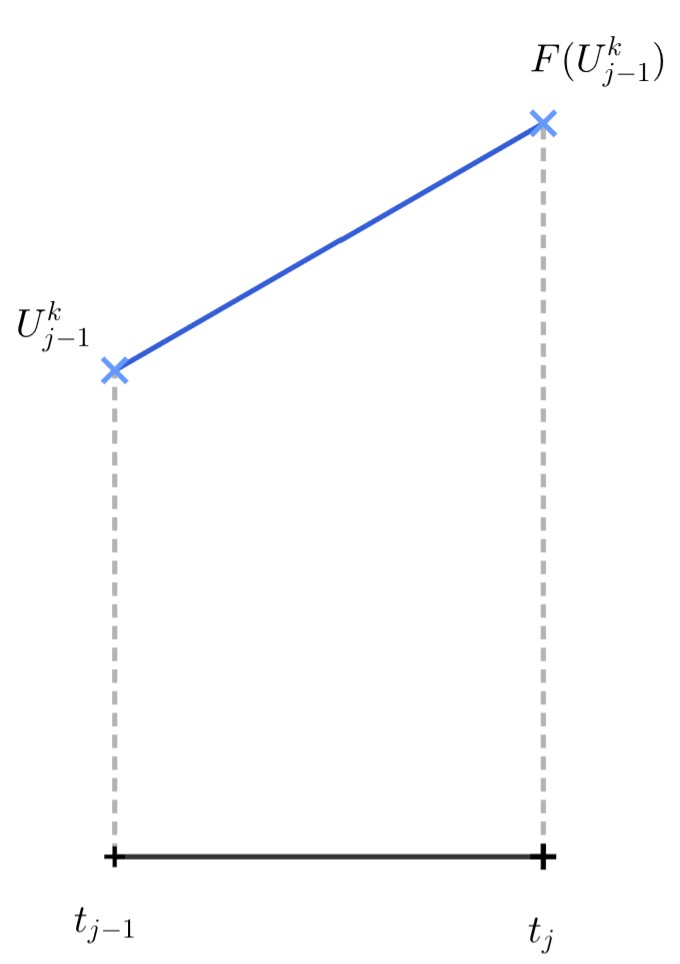
\includegraphics[width=0.4\linewidth]{images/parareal/explane_F.jpg}
	\end{minipage}
	\begin{enumerate}[\textbullet]
		\item $F(U_{j-1}^k), j\in\{1,\dots,P\}$ : value of the fine integrator at $t_j$ starting by $U_{j-1}^k$ (resp. $G(U_{j-1}^k)$)
	\end{enumerate}
	
\end{frame}